\subsection*{Data acquisition}
We recorded the calcium activity  of dense populations of neurons in the supragranular layers in primary visual cortex of anesthetized mice using fast random-access 3D scanning two-photon microscopy \cite{Stosiek:2003,Reddy:2005}.  Numerious repetitions of full-field drifting gratings (Fig. 1A and 1B) were presented to the eye contralateral to the imaged site. This technique allowed recording from a large number (150--350) of cells in a small volume of cortical tissue ($200\times200\times100$ $\mu$m$^3$) in layers 2/3 and 4. Somatic calcium signals were deconvolved using  sparse nonnegative deconvolution \cite{Vogelstein:2010} (Fig.\;1C and 1D).  The average stimulus response was subtracted to remove stimulus covariance and the sample noise covariance matrix was computed (Fig.\;1E).

\begin{figure}[!ht]
\begin{center}
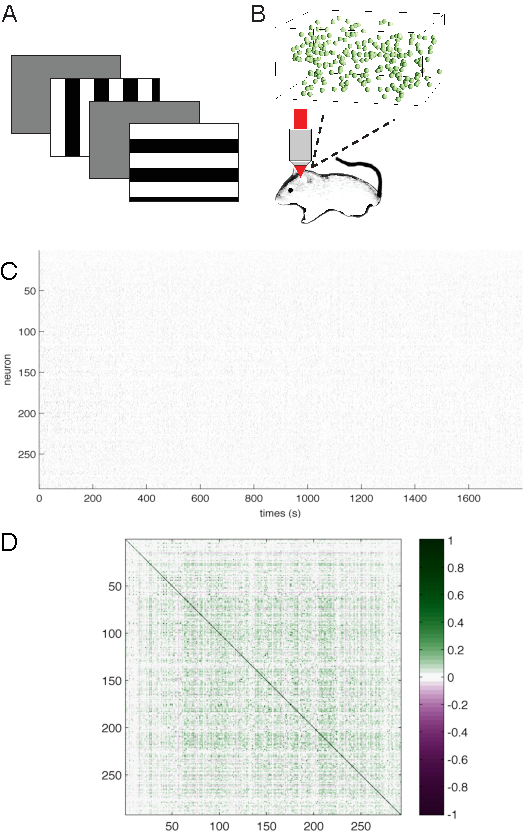
\includegraphics[width=4in]{figures/Figure1.pdf}
\end{center}
\caption{
{\bf Acquistion of neural population activity using two-photon fluorescence imaging of calcium signal.}  {\tt A.} Visual stimuli comprising brief (500 ms) presentatios of full-field drifting gratings separated by blank screens. {\tt B.} Two-photon fast 3D imaging of calcium signals in an awake mouse. {\tt C.} Deconvolved calcium signals. {\tt D.} The sample covariance matrix of neuronal calcium signals in 200 ms time bins. 
}
\label{Figure_label}
\end{figure}


\subsection*{The sample covariance matrix}
We aim to estimate the true covariance matrix $\Sigma = \E{(x-\mu)(x-\mu)^\T}$ of the instantaneous activity vector $x$ of a population of $p$ neurons. Here $\E{\cdot}$ denotes expectation \TODO{for the true data generating process} and $x$ is the $p\times 1$ vector of real-valued instantaneous firing rates discretized into bins of duration $\Delta t$ and $\mu = \E{x}$.  

For more rigorous notation, definitions, and derivations, see Appendix. 

The usual estimator of $\Sigma$ is the sample covariance matrix
\begin{equation}
\hat \Sigma_0 = \frac 1 \nu \sum\limits_{t=1}^n (x(t)-\mu)(x(t)-\mu)^\T 
\end{equation}
where $x(t),\;t=1,\ldots,n$ are sequential observations of population activity inferred from calcium signals; $\nu$ is the number of degrees of freedom. For independent observations $\nu=n-1$ because estimation of the mean $\mu$ accounts for one degree of freedom. When observations are correlated, as is the case with calcium signals, $\nu < n-1$ and may be estimated from the signal. 

The sample covariance matrix is constructed to be unbiased, such that $\E{\hat\Sigma_0} = \Sigma$. 

\subsection*{Evaluation of covariance matrix estimates}
The quality of a covariance matrix estimate $\hat\Sigma$ is measured by a real-valued \emph{loss function} $\loss{\hat\Sigma,\Sigma}$.  The loss function quantifies the deviation of $\hat\Sigma$ from $\Sigma$ and attains its minimum  when $\hat\Sigma = \Sigma$. 

For the purposes of this study, we adopted the \emph{negative normal log-likelihood loss} function:
\begin{equation}\label{eq:loss}
\loss{\hat\Sigma,\Sigma} = \frac 1 p\left[\ln \det \hat \Sigma + \Tr(\hat \Sigma^{-1}\Sigma)\right]
\end{equation}
This choice is motivated by mathematical convenience. Other popular choices for the loss function are the Frobenius norm of the difference $\hat\Sigma-\Sigma$, Stein's entropy loss, and quadratic loss \cite{James:1961,Ledoit:2004,Schafer:2005,Fan:2008}.  We assert that the main conclusions of our study are unlikely to change drastically other well behaved loss functions.

The aim of our project is produce covariance matrix estimates that minimize the expected loss.  The expected loss of an estimator is known as its \emph{risk}: 
\begin{equation}
r = \E{\loss{\hat\Sigma, \Sigma}}
\end{equation}

In practice, the true value $\Sigma$ is not accessible and estimators' risks must be estimated from the data.  This may be accomplished through validation: 
Let $\hat\Sigma_0^\prime$ denote a sample covariance matrix measured from an independent sample that was not used included in the computation of $\hat\Sigma$. Then \emph{empirical loss} is 
\begin{equation}
\hat \ell = \loss{\hat\Sigma,\hat\Sigma_0^\prime}
\end{equation}
 and its expected value or \emph{empirical risk} is
\begin{equation}\label{eq:empiricalRisk}
\hat r = \E{\hat\ell} = \mathbb E_{\hat\Sigma} \left[ \mathbb E_{\hat\Sigma_0^\prime} \left[ {\loss{\hat\Sigma,\hat\Sigma_0^\prime}} \right] \right]
\end{equation}
Because the chosen loss function is linear in its second argument in the sense that
\begin{equation}
\loss{\hat\Sigma,X_1} + \loss{\hat\Sigma,X_2} \equiv \loss{\hat\Sigma,X_1+X_2}
\end{equation}
the expection on the second argument in Eq.~\ref{eq:empiricalRisk} may be taken inside the loss function:
\begin{equation}
\hat r = \E{\loss{\hat\Sigma,\E{\hat\Sigma_0^\prime}}}  = \E{\loss{\hat\Sigma,\Sigma}} = r
\end{equation}
Thus the empirical loss $\loss{\hat \Sigma,\hat \Sigma_0^\prime}$ serves as an unbiased estimate of risk $r$. 

Because the loss function is equivalent to the negative normal log likelihood, the above derivation led us to the familiar criterion that the optimal covariance matrix estimator is one that consistently maximizes the normal log likelihood of the validation dataset.

\subsection*{Regularization}
Under many loss functions\footnote{
The strict equality in Eq.~\ref{eq:bias-variance} does not hold under the loss function in Eq.~\ref{eq:loss}. However, the equality does hold for its close cousin, Stein's \emph{entropy loss},  which only differs by the order of its arguments and a constant offset: $\mathcal L_s(\hat\Sigma,\Sigma) \equiv \loss{\Sigma,\hat\Sigma} - \loss{\Sigma,\Sigma}$. This defficiency presents no difficulty because we minimize the risk directly, without assessing the two error components individually. The bias-variance decomposition is presented here to motivate the use of regularization.}, 
the estimator's risk can be decomposed as the sum
\begin{equation}\label{eq:bias-variance}
r = b + \varepsilon
\end{equation}
of \emph{approximation error} (``bias'' or systematic error)
\begin{equation}
b = \loss{\bar\Sigma,\Sigma}
\end{equation}
and \emph{estimation error} (``variance'') 
\begin{equation}
\varepsilon = \E{\loss{\hat\Sigma, \bar\Sigma}}
\end{equation}
where $\bar\Sigma = \E{\hat\Sigma}$ is the expected value of the estimate. 

The unbiased estimator $\hat\Sigma_0$ makes $\bar\Sigma=\Sigma$ and thereby minimizes the approximation error, but may be excessively susceptible to sample noise and result in high estimation error.

The estimator risk can be reduced by \emph{regularization}. Regularization is the deliberate biasing (\emph{``shrinkage''}) of the estimate toward a low-dimensional, less variable \emph{target estimate} \cite{Bickel:2006,Ledoit:2004}. A regularized estimator solves the bias-variance tradeoff to produce a biased but less variable estimates aiming to minimize the estimator's risk.  Various regularization schemes focus on the dimensionality reduction part \TODO{rephrase} by selecting the optimal target estimate from a family of estimates with reduced dimensionality \cite{findit}.  Other estimators only shrink the sample covariance matrix toward a single target estimator \cite{Schafer:2005}. Yet other regularizers effectively combine shrinkage and dimensionality reduction \cite{findit}.

\subsection*{Estimator A: Shrinkage toward diagonal}
The most popular covariance regularization schemes use diagonal target estimates and linear shrinkage toward the target.  For example, the target could be the identity matrix:  
\begin{equation}
\hat T = \hat v I
\end{equation}
where $\hat v = \frac 1 p \sum\limits_{i=1}^p(\hat\Sigma_0)_{ii}$ is the mean sample variance. 

Alternatively, the target could contain the sample variances:
\begin{equation}
\hat T= \hat\Sigma_0 \circ I 
\end{equation}
where $\circ$ is the entrywise matrix product.

Finally, the target could be a linear mixture of the common variance and independent variance targets
\begin{equation}
\hat T_{\hat\eta} = (1-\hat\eta)(\hat\Sigma_0 \circ I) + \hat\eta\hat v I
\end{equation}

The regularized estimator is the linear mixture of $\hat\Sigma_0$ and $\hat T_{\hat\eta}$:
\begin{equation}
\hat\Sigma_{\hat\eta,\hat\lambda} = (1-\hat\lambda)\hat\Sigma_0 + \hat\lambda \hat T_{\hat\eta} 
\end{equation}

The hyperparameters $\hat\eta$ and $\hat\lambda$ must be estimated from the data.  Under the MSE loss function $\mathcal L_e$ (\ref{eq:MSE}), the optimal values of $\hat\eta$ and $\hat\lambda$ can be estimated analytically \cite{Ledoit:2004,Schafer:2005,Schaefer:2010}. However, these estimates are no longer optimal under the Gaussian loss $\mathcal L_g$. \TODO{I have tested this and there was a substantial difference in both synthetic and empirical data}  When an analytical solution for optimal hyperparameters is not available, the optimal values can be found by cross validation, entirely within the the training sample. \TODO{explain nested cross-validation in more detail?} \TODO{KJ: Yes - see above.}

\TODO{KJ: I am confused.  This suggests that you are getting different results using the two different loss functions.
However, there was no argument yet that either gives us more relevant information about the underlying distribution
if we do not assume Gaussianity, for instance.  I would argue that the Gaussian loss is better, but this is simply 
because the Euclidean metric is not appropriate on the cone of positive semidefinite variances.  As the 
discussion we have been having with Alex demonstrates, this is a point that needs to be explained clearly.}

\TODO{Describe how the empirical loss is convex in the hyperparameters in this case}

\subsection*{Estimator B: Shrinkage toward a factor model}
For estimator B, the target is a factor model, composed as the sum of a low-rank component $\hat L_{\hat d}\hat L_{\hat d}^\T$ and a diagonal matrix $\hat \Psi$:
\begin{equation}
\hat T_{\hat d} = \hat L_{\hat d} \hat L_{\hat d}^\T + \hat\Psi
\end{equation}
Here $\hat L_{\hat d}$ is an $p\times\hat d$ matrix and $\hat\Psi$ is diagonal.  

If $F$ were assume to be multivariate normal \TODO{or other distributions that are defined by linear dependencies}, the factor model is corresponds to the graphical model (\ref{fig:02}B) where the activity of all neurons are dependent only $\hat d$ latent units. This suggest a mechanistic interpretation in which the interactions between neurons are insignificant compared to the influence of inputs outside the recorded circuit.

Just as with Estimator A, Estimator B is allowed to commit to the low-dimensional target only partially: the overall estimate is the linear mixture of the sample covariance and the target
\begin{equation}
\hat\Sigma_{\hat d,\hat\lambda} = (1-\hat\lambda)\hat\Sigma_0 + \hat  T_{\hat d}
\end{equation}

\TODO{Check \cite{Ledoit:2003,Fan:2011,Fan:2006}}

\subsection*{Estimator C: Sparse inverse}
Assuming that $x$ is distributed normally, the inverse of the covariance matrix or \emph{precision matrix} $K=\Sigma^{-1}$ has special significance: zeros in the precision matrix indicate conditional independence between the corresponding pairs. To see this, let $x=(x_1,\ldots,x_p)^\T \sim g\left(x\cond K\right)$
\begin{equation}
g\left(x\cond K\right) = \frac 1 {Z(K)} \exp\left(-\frac 1 2 \sum\limits_{i=1}^p\sum\limits_{j=1}^p  K_{ij} x_i x_j\right)
\end{equation} 
If $K_{12}\equiv K_{21} = 0$, then the joint distribution of $x_1$ and $x_2$, conditioned on $x_3=a_3,\ldots,x_p=a_p$ can be decomposed as product of independent distributions of $x_1$ and $x_2$: 
\begin{equation}
\begin{split}
g\left( x_1, x_2 \cond K, x_3=a_3,\ldots,x_p=a_p\right) &=
\frac 1 {Z(K)} \exp\left(-\frac 1 2 \sum\limits_{i=3}^p\sum\limits_{j=3}^p  K_{ij} a_i a_j \right)\times
\\
 &  \exp\left( -\frac 1 2\left( K_{11} x_1^2 +  x_1\sum\limits_{i=3}^p K_{1i}a_i \right)  \right)
\\
 &  \exp\left( -\frac 1 2\left( K_{22} x_2^2 +  x_2\sum\limits_{i=3}^p K_{2i}a_i \right)  \right)
\end{split}
\end{equation}


\cite{Dempster:1972,Meinshausen:2006,Friedman:2008}

\subsection*{Estimator D: Sparse inverse with latent units}
\cite{Ma:2013} 



\subsection*{In simulation, estimator selection `recognizes' the covariance structure}
\begin{figure}[htp]
\centering
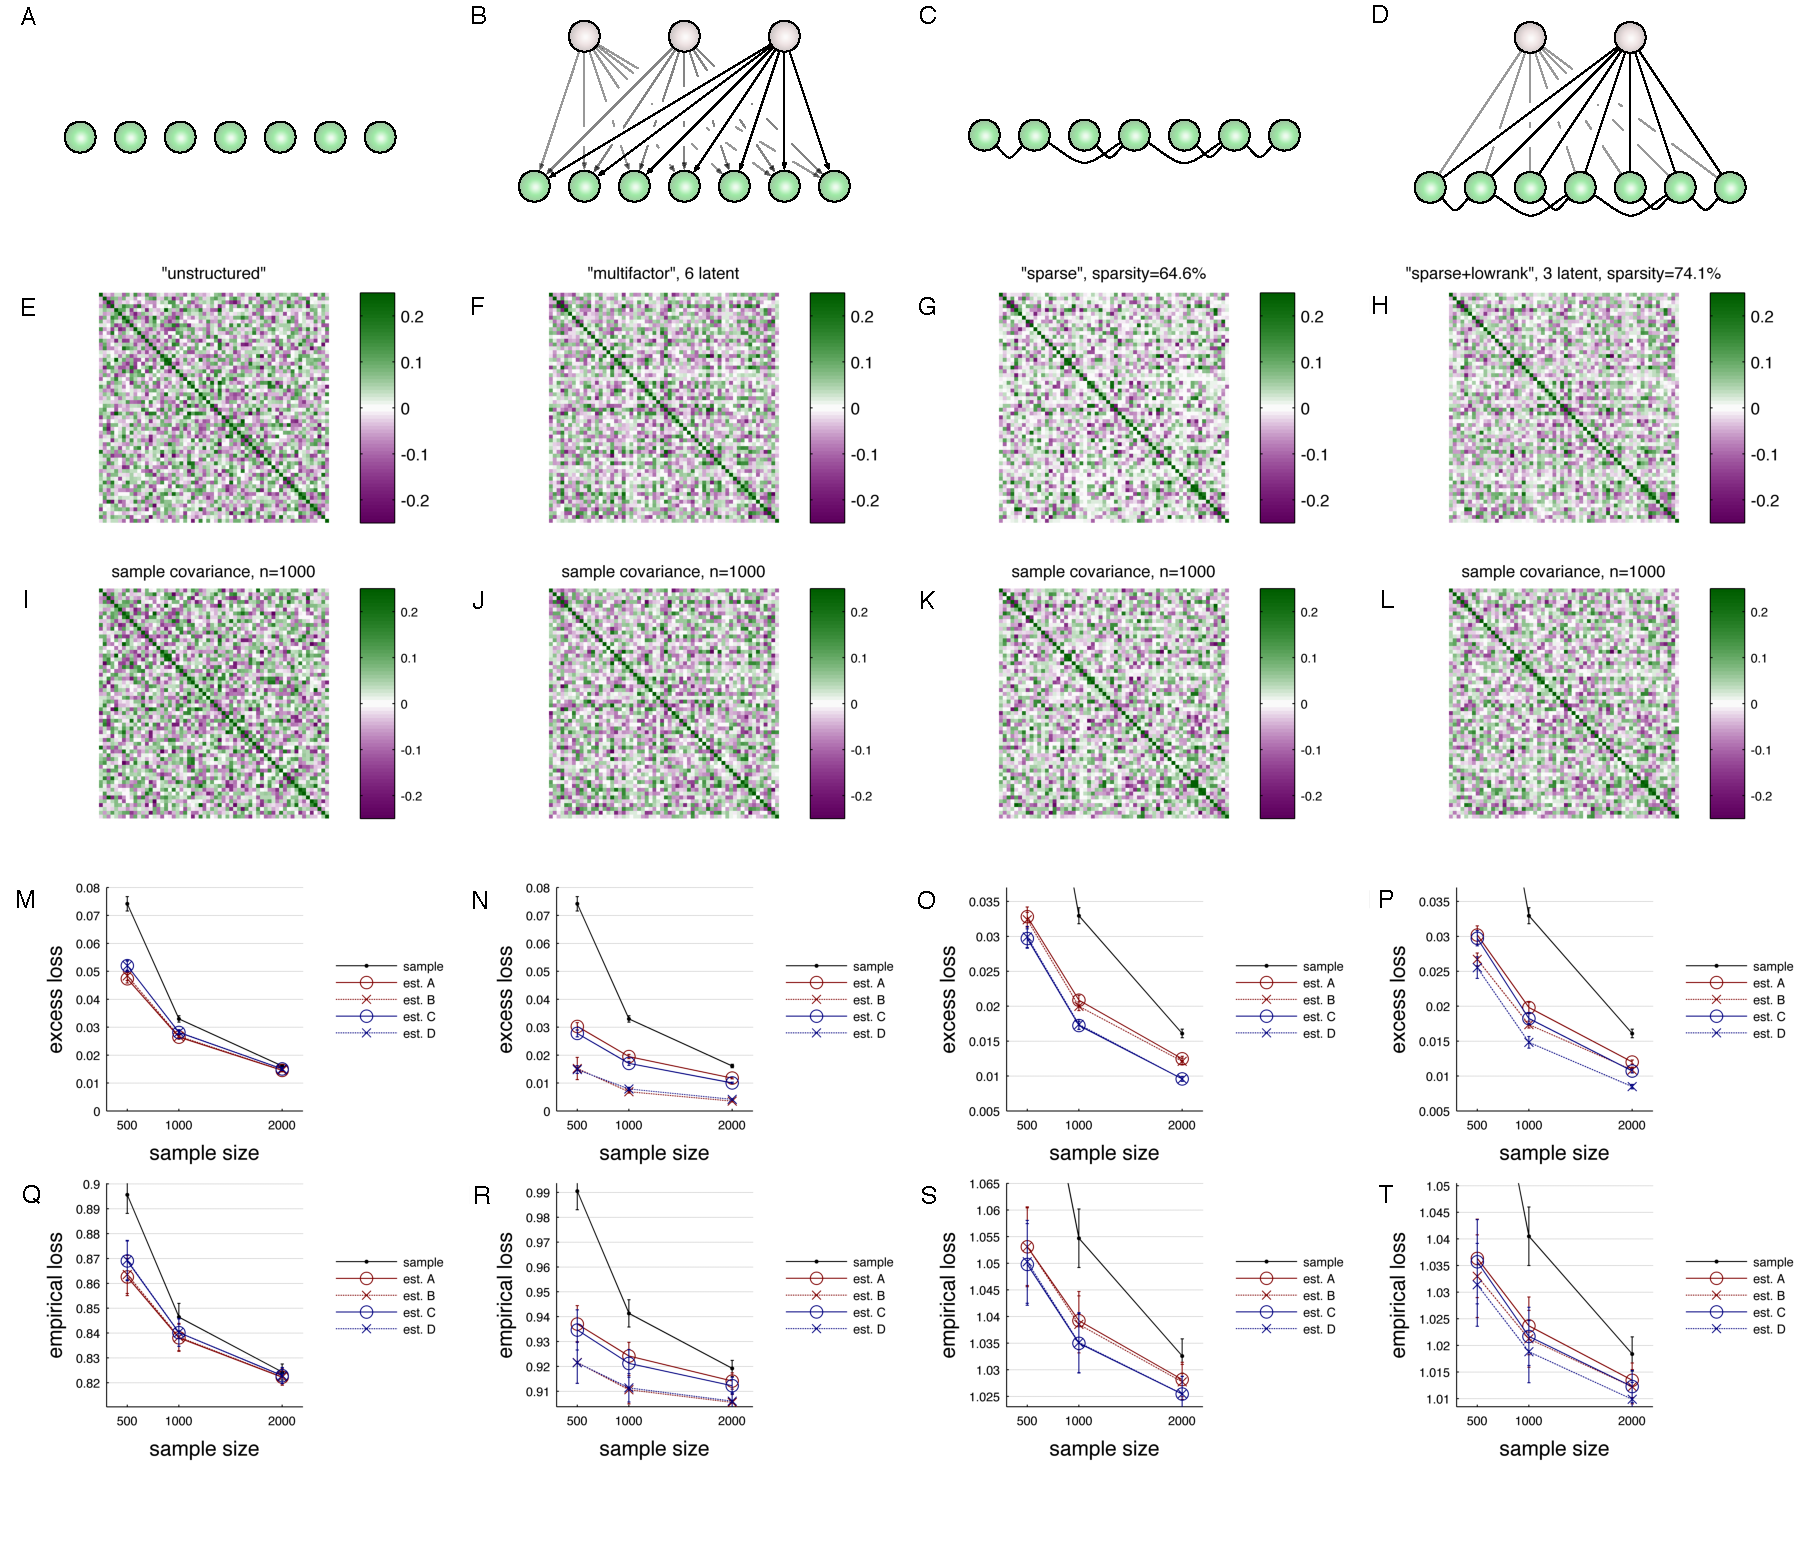
\includegraphics[width=1.0\textwidth]{figures/Figure3.pdf}
\caption{
Selection amongst estimators recognizes covariance atructure.
}\label{fig:03}
\end{figure}


\subsection*{In visual cortex, Estimator D dominates}
\begin{figure}[htp]
\centering
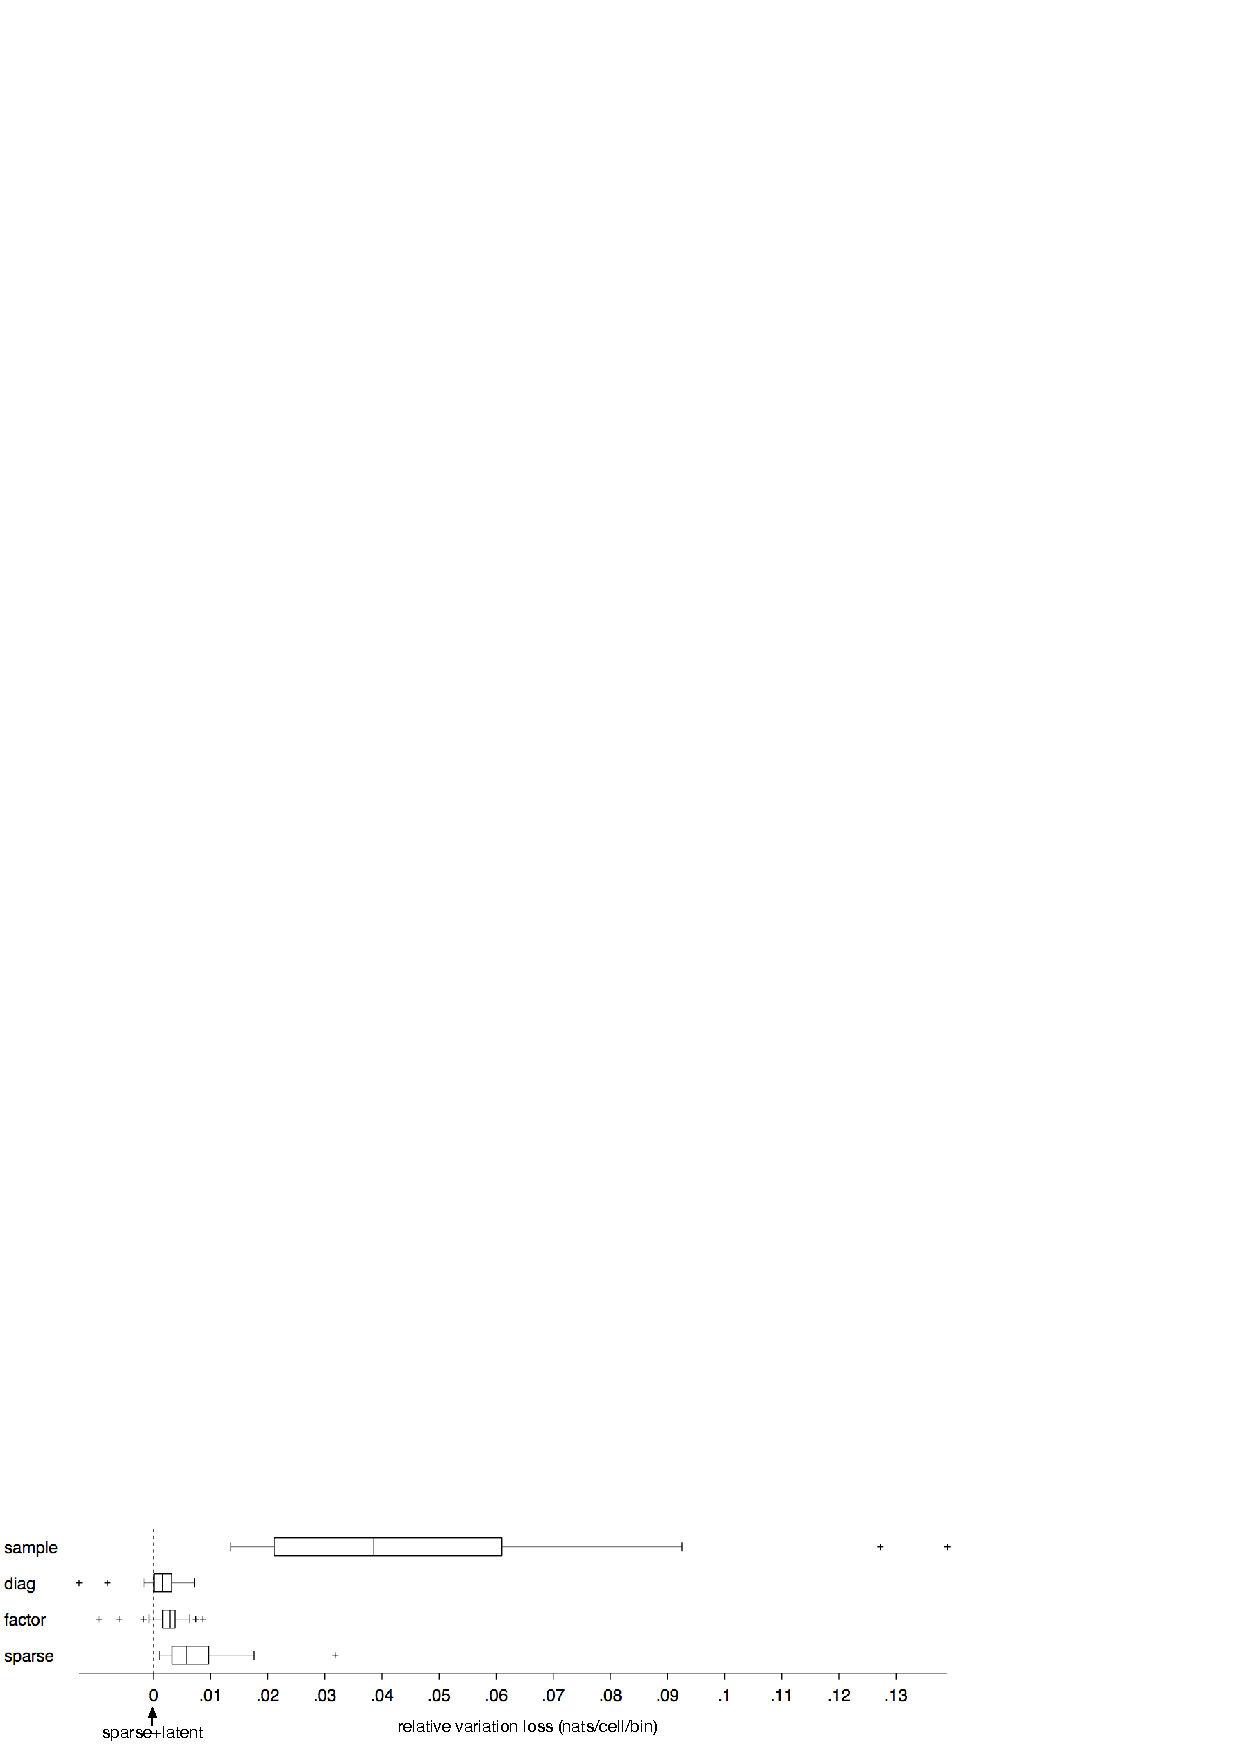
\includegraphics[width=0.5\textwidth]{figures/Figure4.pdf}
\caption{{\bf Estimator $\mathcal D$ (sparse+full-rank inverse covariance) dominates in dense recordings from primary visual cortex.}
{\bf A:}  Histogram of improvements in validation loss by covariance estimator $\mathcal D$ relative to the samle covariance matrix from the 31 imaged sites used in the study.  The vertical red line denotes the median improvment. 
{\bf B:} Improvements relative to estimator $\mathcal A$ (shrinkage toward the diagonal).
{\bf C:} Improvements relative to estimator $\mathcal B$ (shrinkage toward the factor model).
{\bf D:} Improvements relative to estimator $\mathcal C$ (sparse inverse covariance).
}\label{fig:04}
\end{figure}
This is the full matrix of all comparisons of the estimators.  The plots represents the histograms of the differences of the loss function between the pair of estimators for all 31 sites.  When the differences are positive, the first estimate in the title outperforms the second estimate.

Of particular interest is the first row, which shows that all regularized estimates  outperformed the sample covariance estimate.  Even more informative is the last column, which shows that estimate D (sparse+lowrank) significantly outperformed all other estimates.



